\section{Tests}\label{sec:tests}

\subsection{Hernquist model}
To check the correct function of the integration routine, we used the
analytic formulas from \cite{Hernquist1990}:

\begin{eqnarray}
M(r) &=& M\frac{r^2}{(r+a)^2}\\
\nu(r) &=& \frac{M}{2\pi}\frac{a}{r}\frac{1}{(r+a)^3}\\
\beta(r) &=& 0
\end{eqnarray}

with mass scale $M$ and length scale $a$ as inputs, and calculated
$\siglos(r)$ with our numerical routine, including three
integrations. Working with extrapolations to the first bin turns out
to give the most stable results, corresponding nicely to the analytic
value \bcite{BaesDejonghe2002} of

\begin{eqnarray*}
\siglos(r) &=& \frac{1}{I(r)}\frac{1}{24\pi(1-r^2)^3}\times\\
           && \qquad [3r^2(20-35r^2+28r^4-8r^6)X(r) \\
           && \qquad + (6-65r^2+68r^4-24r^6)]-\frac{r}{2},\\
\sigma_r(r) &=& r(1+r)^3 \ln\left(\frac{1+r}{r}\right)\\
 &&\qquad-\frac{r(25+52r+42r^2+12r^3)}{12(1+r)},\\
I(r) &=& \frac{1}{2\pi}\frac{(2+r^2)X(r)-3}{(1-r^2)^2},\\
X(r) &=& \begin{cases}(1-r^2)^{-1/2} \text{arcsech}\,r,& \text{for}\,0\leq r\leq 1,\\
                (r^2-1)^{-1/2} \text{arcsecans}\,r,& \text{for}\,1\leq r\leq\infty
                \end{cases}.
\end{eqnarray*}



A single component model is set up according a simple Dehnen split
power-law sphere \cite{Read+2006},

\begin{equation}
\rho(r) = \frac{M_\infty(3-\gamma)}{4\pi r_S}\left(\frac{r}{r_S}\right)^{-\gamma}\left(1+\frac{r}{r_S}\right)^{4-\gamma},
\end{equation}

where $M_\infty=1$ denotes the total mass, $\gamma=1$ the logarithmic
central asymptotic slope, and $r_S=1$ the scale length. We use $10^6$
sample points, outof which $10^4$ are extracted for further analysis.

We then let $\nu, \rho, \beta$ vary. The MCMC correctly recovers the
underlying mass distribution.



\subsection{Data quality}
How many tracer stars are needed to determine the overall density
profile reliably? To address this question, we performed three runs
with a restricted set of tracer particles. In the first, $10^3$
particles were chosen out of the $10^6$ simulated particles. With
$10^4$ particles, the confidence intervals shrink. These $10^4$
particles are split then into two populations of each $5\cdot10^3$
particles, with different scalelengths of $r_S$ and $r_S/10$. Most of
the second population particles are inside the first two bins, so the
overall convergence is not visibly affected above the third bin.
However, the models are better constrained around the scalelengths of
both tracer populations. This is expected from
\citet{WalkerPenarrubia2011}, as any velocity anisotropy sampling
yields the same mass constraint there.


\begin{figure*}
\begin{center}
\hspace{-7mm}
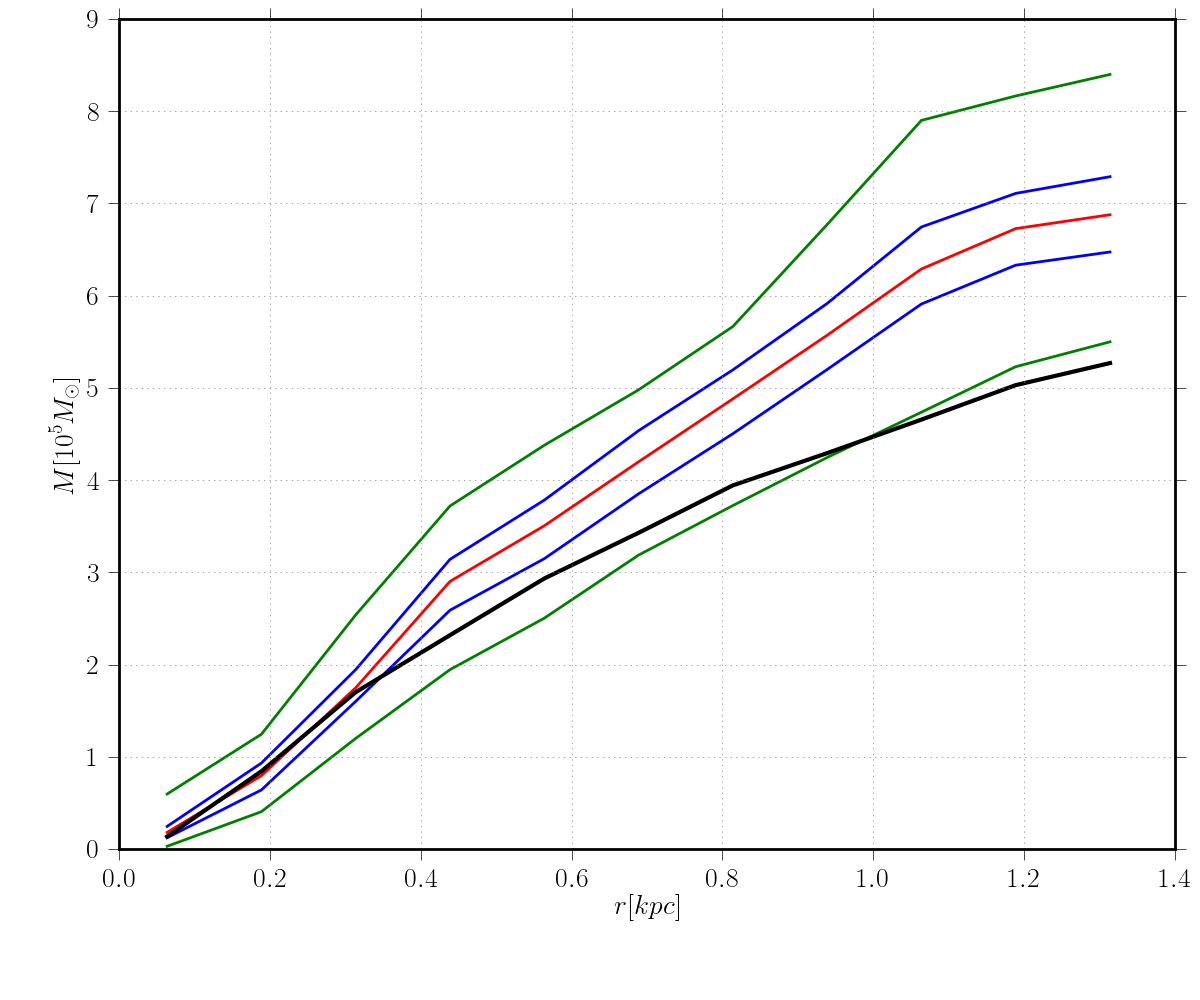
\includegraphics[width=0.3\textwidth]{fig/hernquist1e3.eps}
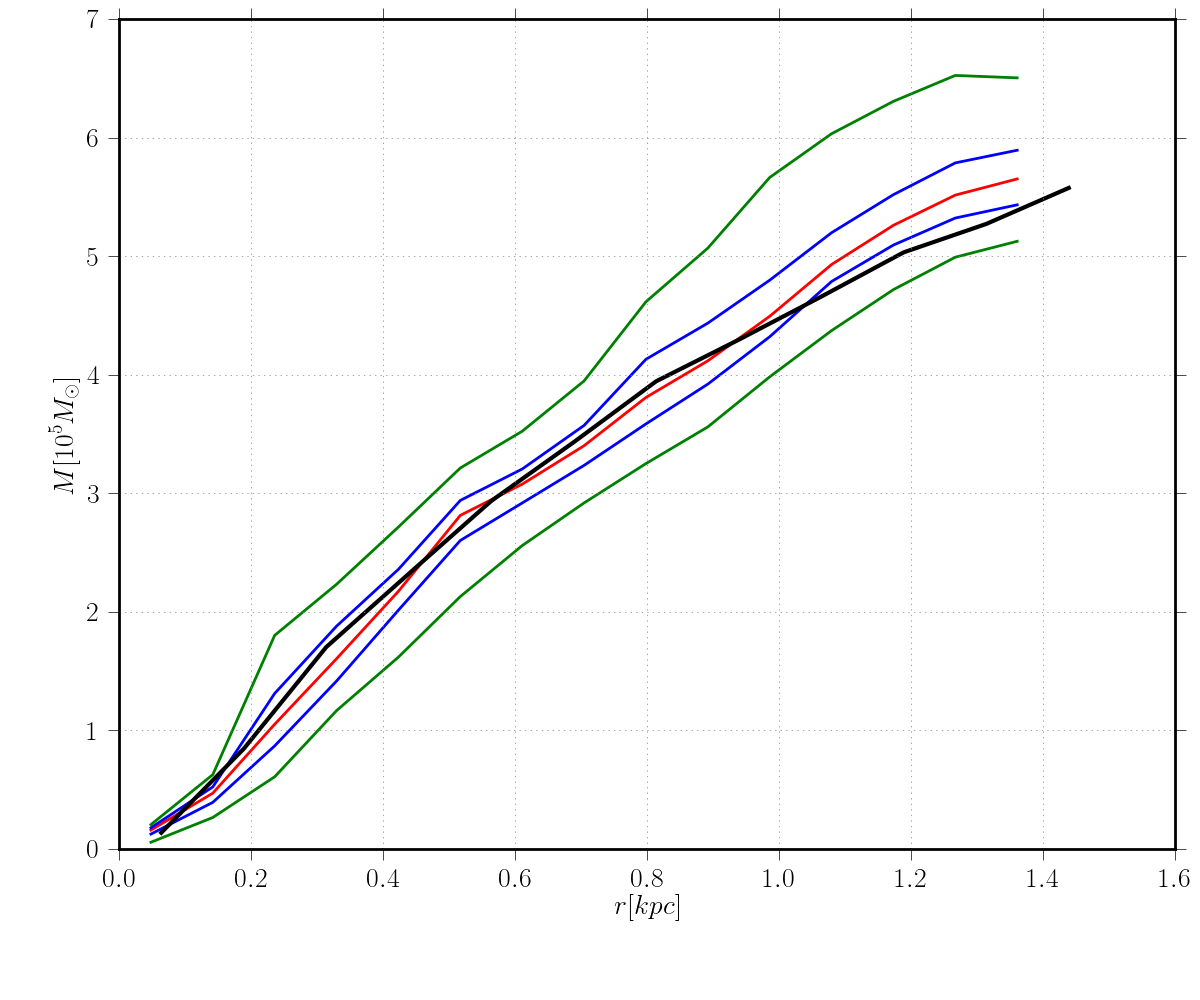
\includegraphics[width=0.3\textwidth]{fig/hernquist1e4.eps}
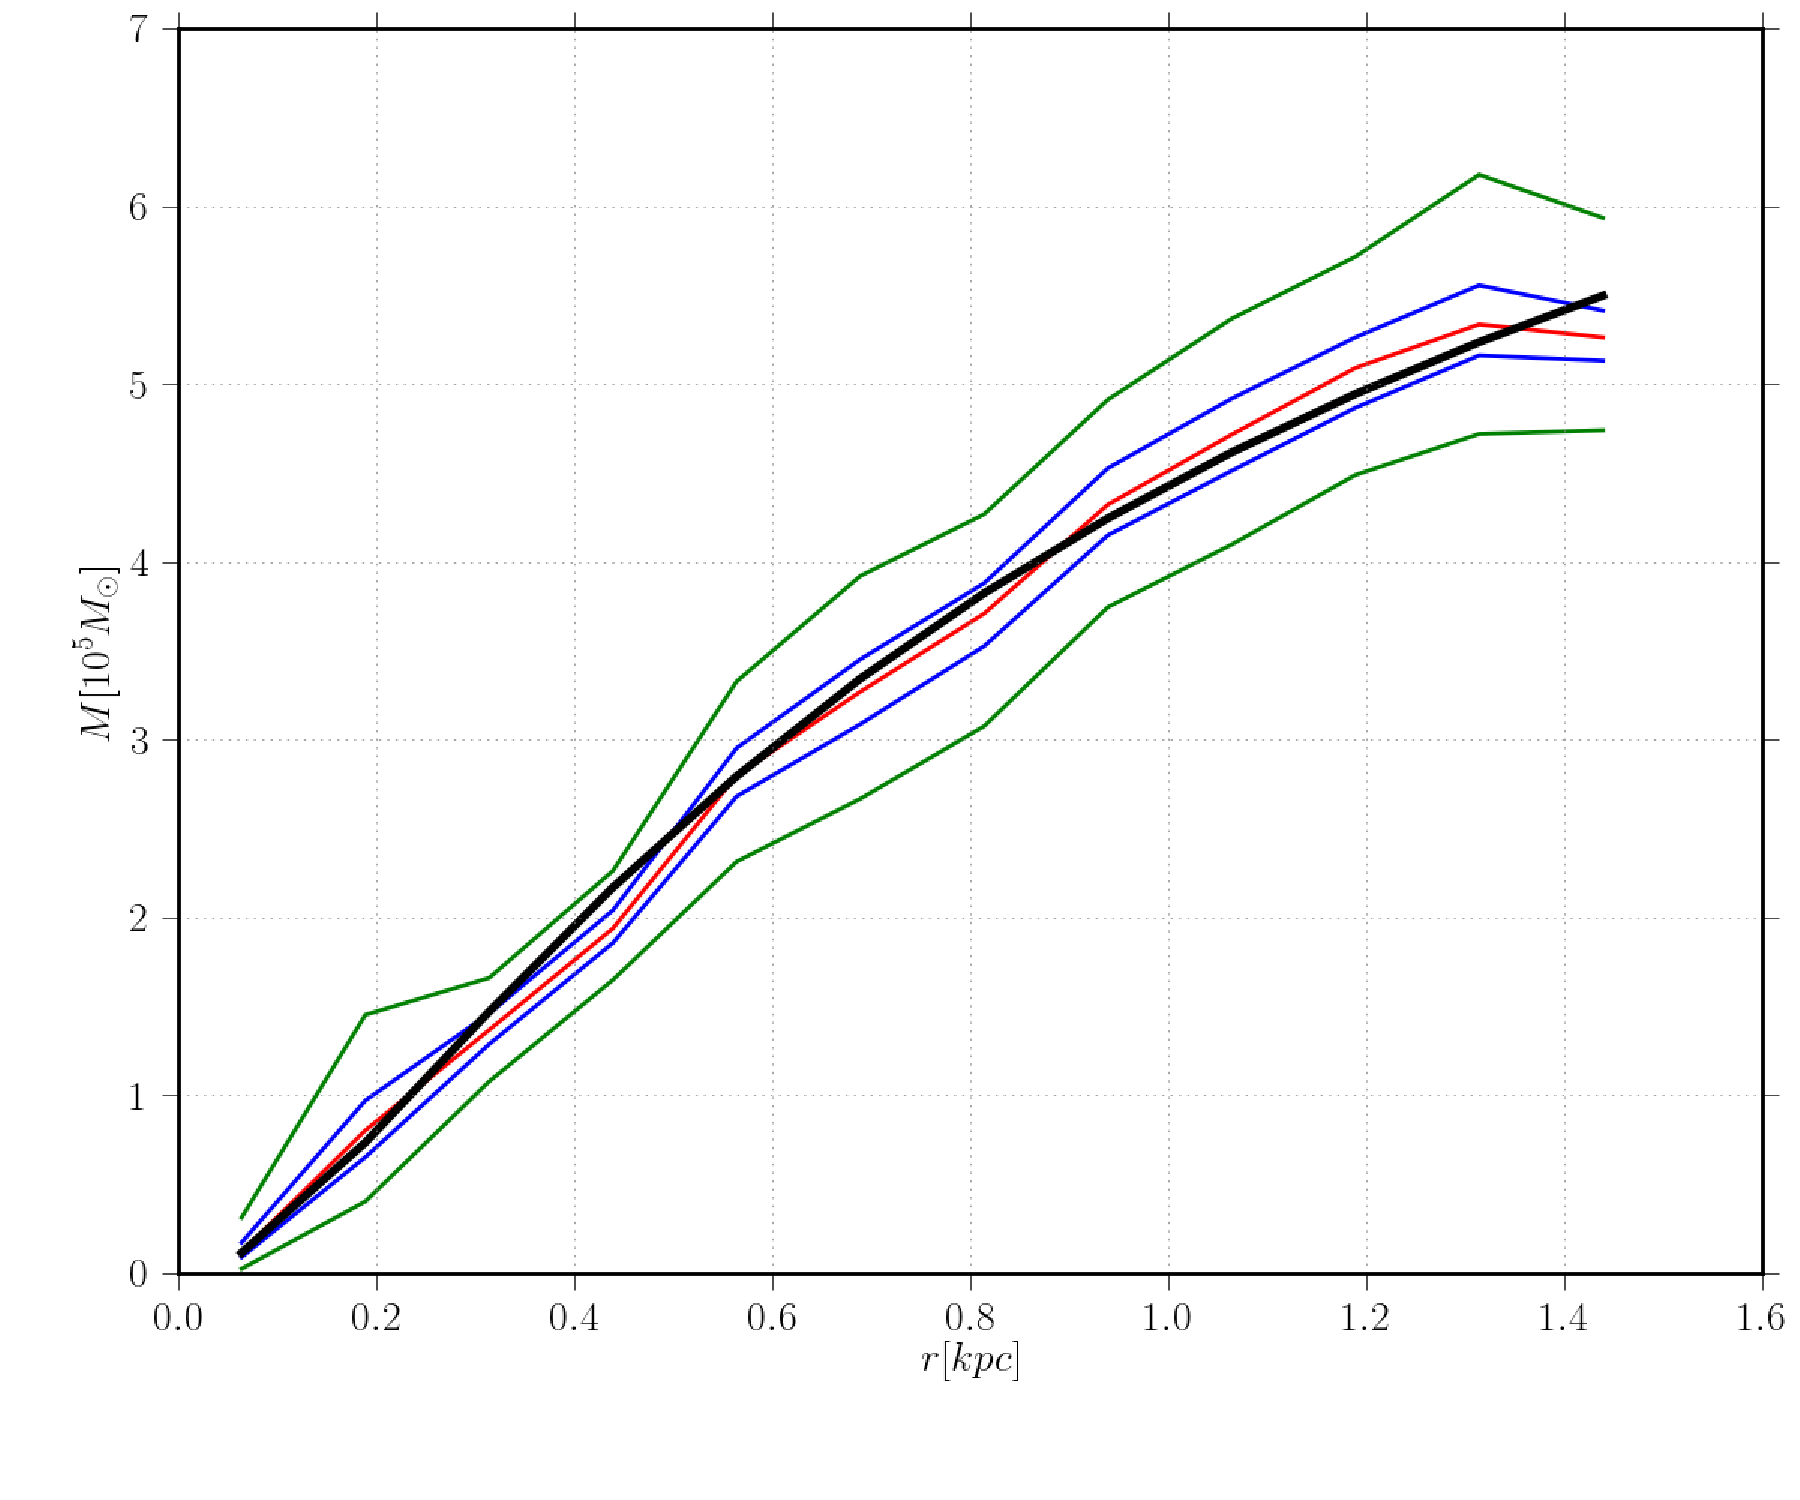
\includegraphics[width=0.3\textwidth]{fig/hernquist2x5e3.eps}
\caption{Hernquist profile found by MCMC model (red) for $10^3$,
  $10^4$ and 2 times $5\cdot10^3$ tracer particles. Black curve
  shows the enclosed mass derived from model.}
\label{fig:hernquist1e3}
\end{center}
\end{figure*}


